UMTS (Universal Mobile Telecommunications System) è stata la prima tecnologia 3G. 
La novità principale rispetto al GSM è nella RAN, dove viene introdotta una nuova interfaccia CDMA (Code Division Multiple Access) e il soft handover.
La core network è molto simile a quella del GSM/GPRS, sia in termini di funzionalità che di procedure di signaling.
Inoltre, viene introdotto il ocncetto di bearer service.
\begin{figure}[H]
	\centering
	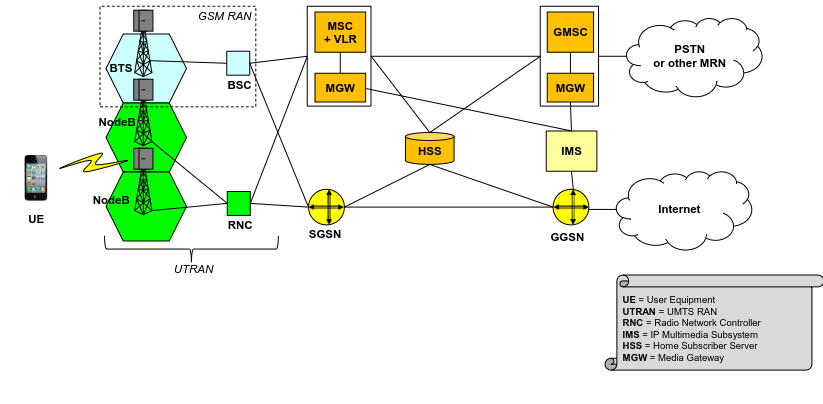
\includegraphics[width=\textwidth]{pictures/10/architettura.png}
	\caption{Architettura di UMTS}
\end{figure}
La rete di accesso ora viene chiamata UTRAN (UMTS Terrestrial Radio Access Network) 
e la core network è pianificata in modo di muoversi verso un'architettura completamente IP.
Ora vediamo le principali componenti di UMTS.
\begin{itemize}
	\item \textbf{User Equipment (UE)}: è l'equivalente di MS
	\item \textbf{Node B}: è l'equivalente di BTS
	\item \textbf{Radio Network Controller (RNC)}: corrisponde a BSC, ma è più complesso e gestisce più funzioni (gestione risorse radio e alcune funzionalità di gestione mobilità)
	\item \textbf{Home Subscriber Server (HSS)}: rimpiazza l'HLR e l'AUC
	\item \textbf{IP Multimedia Subsystem (IMS)}: permette di stabilire delle sessioni (chiamate) tra terminali IP, usa il signaling SIP
	\item \textbf{Media Gateway (MGW)}: permette di interconnettere la rete UMTS con altre reti (PSTN, GSM, ecc.).
	Potrebbe interfacciarsi con un Media Gateway Controller (MGC) che controlla le funzionalità di signaling (spesso viene implementato nel IMS)
\end{itemize}
\section{Miglioramenti}
I miglioramenti apportati hanno reso possibile offrire servizi che hanno bisogno di velocità maggiori.
La prima versione di UMTS offriva una velocità massima di 2Mbit/s,
ma con l'introduzione di HSPA (High Speed Packet Access) si è arrivati a 14.4Mbit/s in downlink e 5.8Mbit/s in uplink, tramite migliorie nella codifica, modulazione e dei protocolli.
Con HSPA+ si è arrivati a 42Mbit/s in downlink e 11Mbit/s in uplink, grazie all'introduzione di MIMO (Multiple Input Multiple Output) e introducendo il concetto di flat network.
\bigskip

La UTRAN e la core network hanno la capacità di assegnare le risorse ai canali dati con diverse caratteristiche (velocità, latenza, ecc.) 
a seconda del servizio che si vuole offrire. Questo permette di offrire ottimizzazioni per servizi multimediali.
Viene quindi introdotto il concetto di \textbf{bearer service}.
\section{Bearer services}
Un bearer è un concetto flessibile che indica una "bit pipe" tra entità con determinati attributi di QoS.
È un'estensione del concetto di tunnel definito in GPRS.
Ogni bearer appartiene a un bearer service, dove le entità coinvolte definiscono il tipo di bearer service.
Possono essere definite diverse classi di service in base al QoS richiesto, ad esempio:
\begin{itemize}
	\item Conversational
	\item Streaming
	\item Interactive
	\item Background
\end{itemize}
\begin{figure}[H]MC Zoom 35-70mm f/3.5-4.5 manual
	\centering
	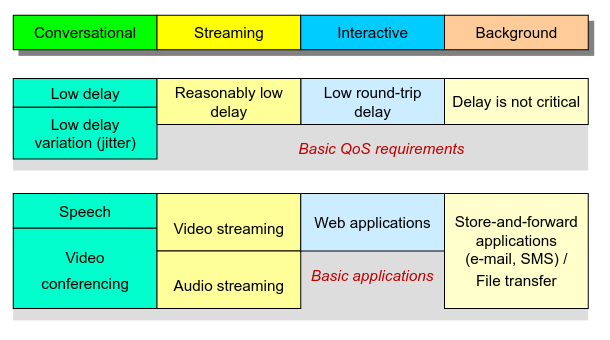
\includegraphics[width=0.7\textwidth]{pictures/10/classi.png}
	\caption{Classi di bearer service}
\end{figure}
Gli attributi di QoS usati per specificare un bearer service sono:
\begin{itemize}
	\item Beatrate massimo
	\item Beatrate minimo garantito
	\item Delay massimo
	\item Probabilità di errore
\end{itemize}
Gli attributi utilizzati dipendono dalla service class, dato che non tutti devono essere specificati per ogni classe.
\bigskip
Ci sono diversi servizi che coinvolgono diversi nodi:
\begin{itemize}
	\item Core Network (CN) bearer service: tra i noti della core network (SGSN e GGSN)
	\item Radio Access Bearer (RAB) service: tra UE e SGSN
	\item Radio Bearer Service: tra UE e RNC
\end{itemize}
Un RAB deve essere sempre stabilito prima che un utente possa iniziare a trasmettere dati, la sua creazione viene richiesta dal SGSN e viene utilizzato sia per i dati che il signaling.
\begin{figure}[H]
	\centering
	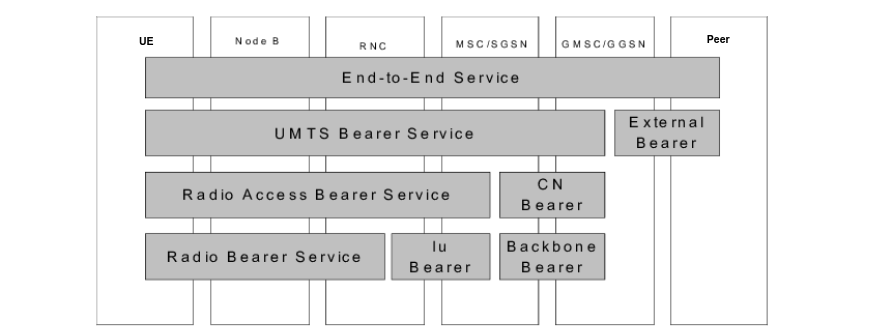
\includegraphics[width=0.9\textwidth]{pictures/10/servizi.png}
	\caption{Tipi di bearer service}
\end{figure}
\section{Soft handover}
Permette agli UE di connettersi a diversi node B contemporaneamente.
Lo stato di soft handover è gestito dalla RNC, che decide quando connettere o disconnettere un node B, fino a un massimo di sei.
Nella direzione di uplink, le trasmissioni vengono ricevute da tutti i node B connessi e il segnale migliore viene selezionato.
Nella direzione di downlink, la RNC invia lo stesso segnale a tutti i node B connessi, che lo trasmettono contemporaneamente, e l'UE mantiene il primo che arriva.
\begin{itemize}
	\item \textbf{Vantaggi}: migliore qualità di comunicazione e nessuna interruzione di servizio
	\item \textbf{Svantaggi}: più risorse allocate
\end{itemize}
\section{Schema di autenticazione}
Cambia rispetto a GSM, dato che l'HLR e l'AUC vengono rimpiazzati da un unico nodo, l'HSS.
\begin{figure}[H]
	\centering
	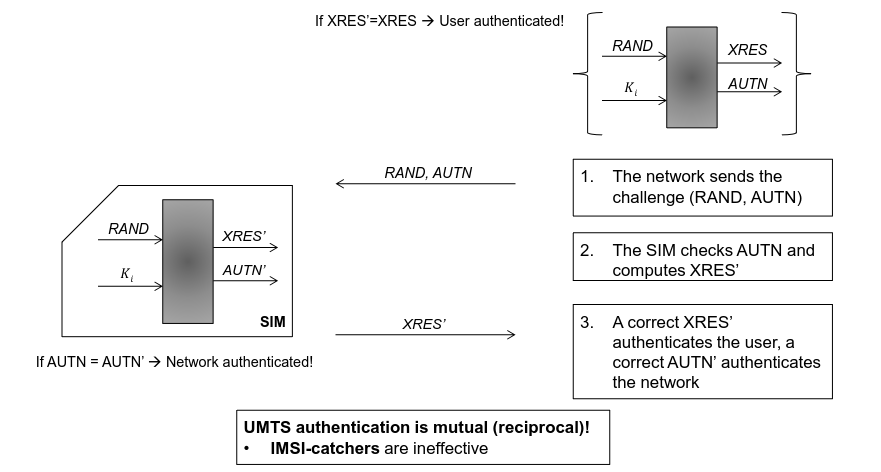
\includegraphics[width=0.9\textwidth]{pictures/10/autenticazione.png}
	\caption{Schema di autenticazione in UMTS}
\end{figure}